\subsection{Communicating hierarchical hybrid \\automata}
\label{HCHA}
{\it As noted in the introduction, the execution of an autonomous plan involves many levels of abstraction. The verification must cover all these levels.}

{\it We use the formalism of hierarchical  communicating hybrid automata (HCHA) to model agents in the scenario. }
We start with a few basic elements:
an agent (of one of the types described above) has a state vector $\stPt \in \reals^n$.
(Different agents may have different dimensions.)
The state includes all information of relevance to the system designers.%: for the ego vehicle, this will typically include position and velocity, but also fuel combustion rate and wall-wetting effects if needed.
%For a traffic light (which is an agent of type \texttt{trafficSignage}), the state might include the current active light and a clock that measures the delay between light switches.
An agent is modeled as a \emph{communicating} hybrid automaton.

\begin{defn}[Communicating hybrid automaton]
	\label{def:CHA}
A driven \textbf{communicating hybrid automaton} (CHA) $\Sys$ with inputs in $\inpSet$ 
is a tuple 
\[\Sys = (\stSet, \modeSet, E, Inv, \{F_\mode\}_{\mode \in \modeSet}, \guard, \reset, \funcOut, C)\]
where 
\begin{itemize}
	\item $\stSet \subseteq \Re^n$ is the continuous state space of the system.
	\item $\modeSet \subset \Ne$ is a finite set of control locations that the system switches through. 
	\item $\hsSet \triangleq \modeSet \times \stSet$ is then the hybrid state space.
	\item $F_\mode : \stSet \times \inpSet \rightarrow \Re^n$ defines a differential inclusion governing the evolution of the state in location $\mode$: $\dot{\stPt} \in F_\mode(\stPt,u)$. 
	\item $Inv : \modeSet \rightarrow 2^\stSet$ defines an invariant condition on the state while in location $\mode$.
	\item $E \subseteq \modeSet \times \modeSet$ is the set of location transitions (a.k.a. switches, or jumps).
	%
	\item $\guard : E \rightarrow 2^\stSet$ is the guard condition that enables a location transition. 
	Namely, the system switches between $\mode _i$ and $\mode _j$ when the state $\stPt$ is in $\guard((\mode_i,\mode _j))$.
	%
	\item $\reset : E \times \stSet \rightarrow \modeSet \times \stSet $ is a reset map that, given a transition $e = (\mode _i,\mode _j) \in E$ and a point $x$ on the guard $\guard(e)$, maps $x$ to a point $x^+$ in the invariant set of the next location $\mode_j$:
	\[\reset: ((\mode _i,\mode _j),x) \rightarrow (\mode_j,x^+)\;, x^+ \in Inv(\mode_j)\] 
	%
	\item $\funcOut: \reals^n \rightarrow \reals^p$ is an output function,
	\item $C = \{c_1,\ldots,c_p\}$ is a set of $p \in \Ne$ perception conditions (defined below).	
\end{itemize}
\end{defn}

The differential inclusion $F_\mode$ in each location of the CHA models the continuous-time closed-loop behavior of the low-level controlled systems, i.e., the electromechanical systems of the car such as the powertrain.
As stated earlier, the state $\stPt$ captures all the relevant information about the agent's dynamics. 
It is widely recognized now that different navigation situations call for different control laws.
\todo[inline]{cite}
This is modeled by the locations of the CHA: each location represents the application of a different control law that is appropriate for the situation.

The solutions of regular ODEs are given as functions of the independent variable time $t$.
Because hybrid automata also include a discrete evolution of the state (namely, via the reset map $\reset$), their solutions will be given as a function of time $t$ and jump number $j$.
We first define hybrid time domains and arcs.
\begin{defn}[Hybrid time domains and arcs~\cite{GoebelT06_SolnsHybInclusions}]
	\label{def:hybridarcs}
	A subset $E \subset \Re_+\times \Ne$ is a \emph{compact hybrid time domain} if 
	\[E = \bigcup_{j=0}^{J-1}[t_j,t_{j+1}]\times \{j\}\]
	for some finite increasing sequence of times $0=t_0 \leq t_1 \leq t_2 \leq \ldots \leq t_J$.
	We say $E$ is a \emph{hybrid time domain} if for all $(T,J) \in E$, 
	$E \cap ([0,T]\times \{0,\ldots,J\})$ is a compact hybrid time domain.
	Define
	$\sup_t E = \sup \{t \sut \exists (t,j) \in E\}$, $\sup_j E = \sup \{j \sut \exists (t,j) \in E\}$,
	and $E.last = (\sup_t E, \sup_j E)$.
	
	A \emph{hybrid arc} $\hstraj$ is a function supported over a hybrid time domain $\hstraj:E \rightarrow \Re^n$, 
	such that for every $j$, $t \mapsto \hstraj(t,j)$ is absolutely continuous in $t$ over $I_j = \{t: (t,j) \in E\}$;
	we call $E$ the domain of $\hstraj$ and write it $\dom \hstraj$.
	%The \emph{graph} of a hybrid arc is the set $\gph \hstraj = \{(t,j,\hstraj(t,j)): (t,j) \in \dom \hstraj\}$.
	Finally, $\dom_t \hstraj = \proj{\dom \hstraj}{\nnreals}$ and $\dom_j \hstraj = \proj{\dom \hstraj}{\Ne}$
\end{defn}

Note that each $I_j$ is an interval.
%$E.last$ indicates the last element of $E$ under the linear order $(t,j) \leq (t',j')$ iff $t \leq t'$ and $j\leq j'$.
As observed in \cite{SanfeliceT10automatica}, hybrid time domains are equivalent to hybrid time trajectories used in \cite{LygerosJSZS03tac} to define executions of hybrid automata.
Output and state trajectories of hybrid automata will be modeled as hybrid arcs. 

Given a hybrid automaton $\Sys$ and a point $\hsPt_0  = (\mode_0, \stPt_0)$, 
a \emph{solution} $\hstraj_{\hsPt_0}$ of $\Sys$ (aka \emph{state trajectory}) is given by a hybrid arc $\hstraj$ 
satisfying the following conditions:
\begin{enumerate}
	\item $\hstraj_{h_0}(0,0) = h_0$
	\item $\hstraj_{h_0}(t,j) = (\mode(t,j),\sttraj(t,j)) \in \hsSet \; \forall (t,j) \in \dom \hstraj$
	\label{item:explicitLX}
	\item For each $j$ s.t. $I_j$ has a non-empty interior, 
	\[\dot{\sttraj}(t,j) \in F_{\mode(t,j)}(\sttraj(t,j))\]
	for almost all $t \in I_j$, and $\sttraj(t,j) \in Inv(\mode(t,j))$ for all $t \in \text{int}I_j$.
	Moreover, 
	\begin{equation*}
	\label{eq:zeroderiv}
	\dot{\mode}(t,j) = 0 \; \forall t \notin \{ \inf I_j, \sup I_j\}
	\end{equation*}
	\label{item:contevolutions}
	\item For all $j$ s.t. $(t,j) \in \dom \hstraj$, $(t,j+1) \in \dom \hstraj$, it holds that $\sttraj(t,j) \in \guard(\mode_i,\mode_k)$ for some $i,k$,
	$\sttraj(t, j+1) = \reset(\sttraj(t,j), (\mode_i,\mode_k))$,
	and $\sttraj(t,j+1) \in Inv(\mode_j)$.
	\label{item:jumpHA}
\end{enumerate}
See Fig.~\ref{fig:HA} for an illustration.
We consider that the discrete time variable $j$ simply counts the location changes (via \eqref{eq:zeroderiv} and Condition \ref{item:jumpHA}).
The transition itself between locations takes 0 real time.
The location changes can only occur when the continuous state $\stPt$ enters a guard set (Condition \ref{item:jumpHA}). 
The sequence of control locations that the trajectory $\hstraj$ visits is denoted by $\loc(\hstraj)$.

If $\hstraj$ is a state trajectory, then $\funcOut \circ \hstraj: \dom \hstraj \rightarrow \hsSet$ is called an \emph{output trajectory}.
We assume that $\funcOut$ is such that an output trajectory is also a hybrid arc, supported on the same hybrid time domain as the corresponding state trajectory:
$\dom \hstraj = \dom \funcOut \circ \hstraj$.

\begin{figure}[tb]
	\centering
	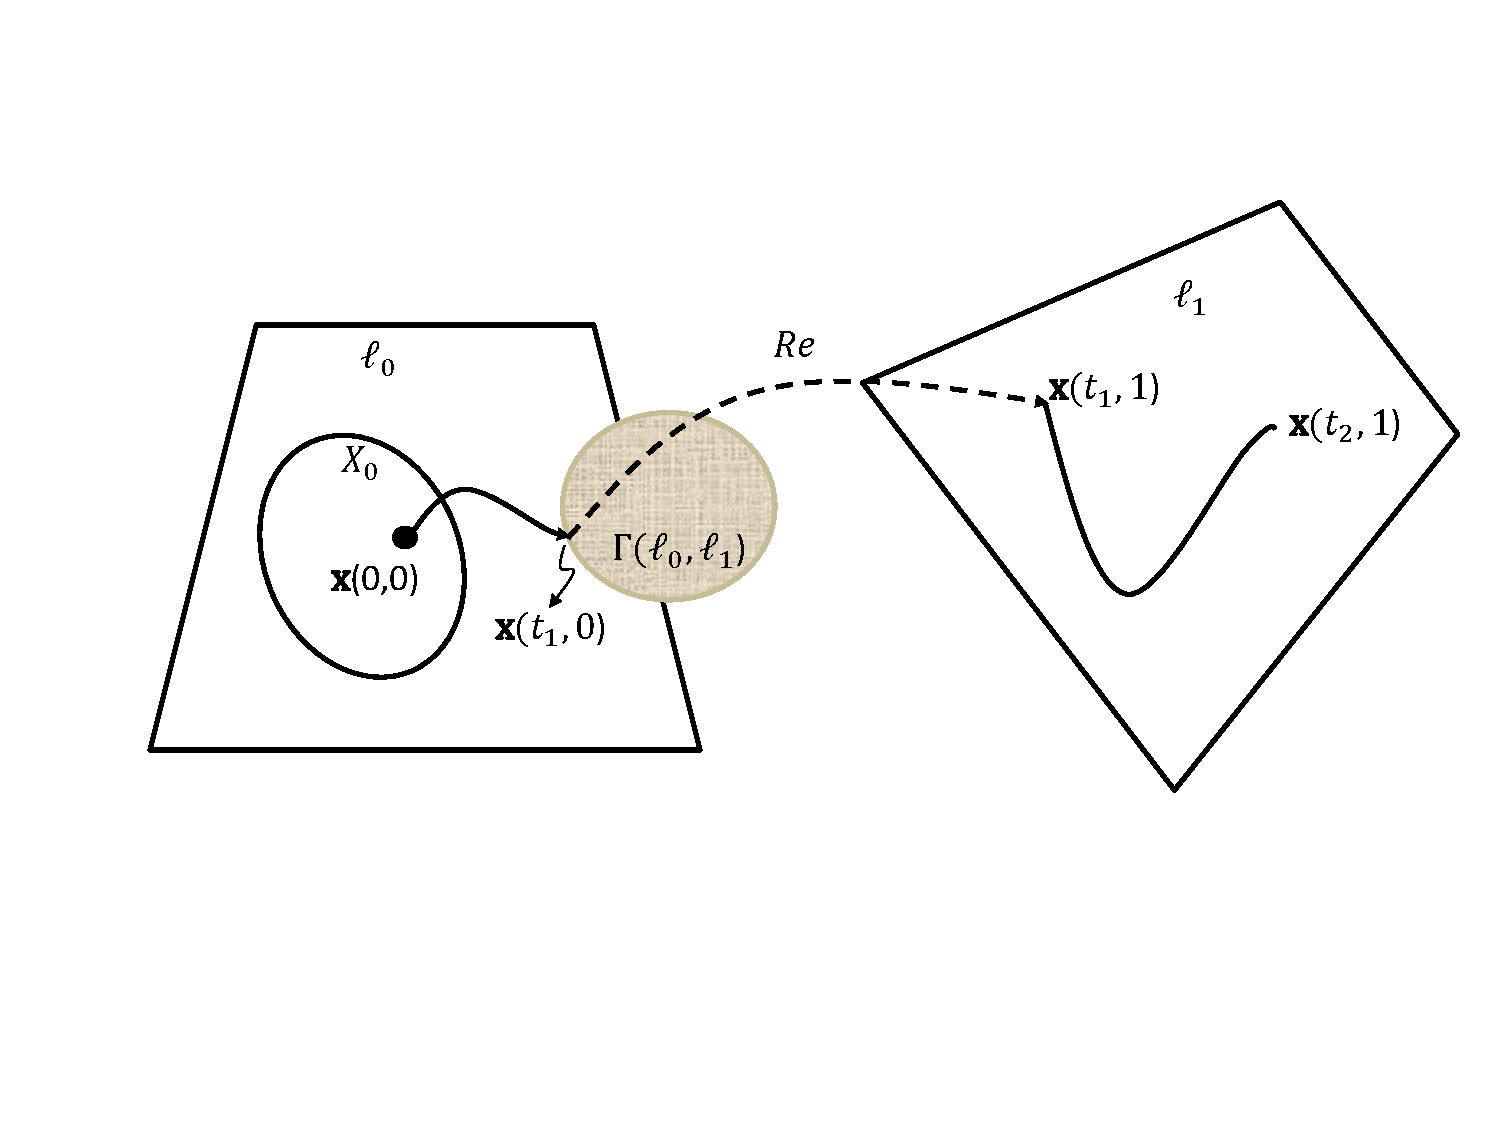
\includegraphics[scale=0.4]{figures/HA.pdf}
	\caption{State trajectory of a hybrid automaton.}
	\label{fig:HA}
\end{figure}

\begin{defn}
	\label{def:solutionsets}
	$\Sc_\Sys(\hsPt_0)$ will denote the set of solutions of $\Sys$ with initial condition $\hstraj(0,0) = \hsPt_0$,
	and $\Sc_\Sys$ will denote the set of all solutions of $\Sys$.
	A hybrid automaton is said to be \emph{deterministic} if $\Sc_\Sys(\hsPt_0)$ is a singleton for any $\hsPt_0$.
\end{defn}

We will use $\hstraj_\hsPt$ to refer to the trajectory starting at $h$.
The system has a finite set of initial locations $\modeSet_0 \subset \modeSet$ in which it could start, 
and within each such location $\mode$, a set of initial continuous states $\stSet_\mode \subset \stSet$ in which it could start. 
Any solution to the system's equations must start there. We denote 
\[H_0 = \bigcup_{\mode \in \modeSet_0} \{\mode\}\times \stSet_\mode\]
the hybrid initial set, and write
\[Init = \bigcup_{\mode \in \modeSet_0}\stSet_\mode \]


\begin{exmp}[Lane change continued]
	We model the lane change scenario using HCHA as follows
	\todo[inline]{must show how the 4 agent types are modeled with this}
	\end{exmp}


\subsubsection{Abstraction levels}
\label{abstractionLevelsOfHCHA}

We formally define the abstraction levels at which it is controlled, and consequently at which it is verified.
A \emph{hierarchical} CHA is a CHA with a chain of partitions defined on its location set $\modeSet$, and a corresponding chain of simplified continuous dynamics.
\begin{defn}[Hierarchical CHA]
	\label{def:HCHA}
	A \textbf{hierarchical CHA} (HCHA) is a tuple 
	$(\Sys, \{V_i\}_{i=0}^{a}, \{P_i\}_{i=0}^{a}, \{\Sys_i\}_{i=0}^{a})$ where 
	$\Sys$ is an $n$-dimensional CHA, 
	each $V_i$ in the chain 
	\[V_a \subset V_{a-1} \subset \ldots \subset V_1 \subset V_0=\{1,\ldots,n\}\]
	is the set of \emph{surviving variables} at level $i$, and 
	$\{P_0,P_1,\ldots,P_a\}$ is an ascending chain of partitions of the set $\modeSet$, that is:
	\begin{itemize}
		\item $P_0 = \modeSet$
		%
		\item For every $i =1,\ldots,a$, $P_i \subset 2^\modeSet$ partitions $\modeSet$: $[\mode] \cap [\mode'] = \emptyset$ for all $[\mode],[\mode'] \in P_i$ and $\cup_{\mode\in \modeSet}[\mode] = \modeSet$
		%
		\item For all $i<a$, for all $[\mode]\in P_i, \exists [\mode'] \in P_{i+1}$ s.t. $[\mode] \subset [\mode']$ 
	\end{itemize}
	Every element of $\{\Sys_i\}_{i=1}^{a}$ is an $n_i$-dimensional CHA 
	\[\Sys_i = (\stSet_i, \modeSet_i, E_i, Inv_i, \{F_{q,i}\}_{q \in \modeSet_i}, \guard_i, \reset_i, \funcOut_i, C_i)\]
	where  $\Sys_0 = \Sys$,
	$n_i \geq n_{i+1}$,
	\begin{eqnarray*}
		\modeSet_i &=& P_i
		\\
		(q,q') \in E_i &\text{ iff }& \exists \mode \in q, \mode' \in q' \text{ s.t. } (\mode,\mode') \in E_{i-1}		
		\\
		\stSet_i & = & \proj{\stSet_{i-1}}{V_i} 
		\\
		\guard_i((q,q')) &=& \proj{\cup_{(\mode,\mode') \in q\times q'} \guard_{i-1}((\mode,\mode')) }{V_i}
		\\
		Inv_i(q) &=& \proj{ \cup_{\mode \in q}Inv_{i-1}(\mode)}{V_i}
		\\
		F_{q,i}(x) &\supset & \proj{\cup_{\mode \in q}F_{\mode,i-1}(x^\uparrow)}{V_i}
		\\
		\reset_i(e,x) &=& \proj{\cup_{e' \subset e}\reset_{i-1}(e',x^{\uparrow})}{V_i}
		\\
		\forall x \in \stSet_{i-1},\; \proj{x}{V_i} &=& \proj{\reset_{i-1}(e,x)}{V_i}
		\\
		C_i &=& C
		\end{eqnarray*}
Finally, for all $ e \in E_{i-1},x \in \guard_{i-1}(e)$,
\[\proj{x}{V_i} = \proj{\reset_{i-1}(e,x)}{V_i}\]
		
\end{defn}
\todo[inline]{should $F$ be the convex hull of the union?}
Every element $P_i$ of the partition chain represents an abstraction level. 
An element $[\mode]$ of $P_i$ is a `super-mode' which aggregates several modes of $P_{i-1}$ (namely, the elements of $P_{i-1}$ in the equivalence class $[\mode]$).
The state vector is reduced in dimension by projecting the state vector at abstraction level $i-1$ onto the variables $V_i$ of the new level. 
The set $V_i$ is part of the data of the HCHA.
For example, it may consist of the state variables that appear in the guard conditions leading out of the super-modes $q \in \modeSet_i$.
The guards and invariants are defined accordingly, by doing the same projection for all guard and invariant conditions on a given transition in $\Sys_{i-1}$.
The new level's dynamics $F_i$ are part of the data of $\Sys_i$. 
For example, they may be obtained by Model Order Reduction from the dynamics of $\Sys_{i-1}$, or some domain-specific transformation.
The input set is correspondingly modified.
Note that by imposing $C_i=C$ we impose that the variables involved in each perception condition survive all levels.
This is a reasonable assumption when we consider that perception conditions involve physical quantities that can be perceived by other agents in the environment, and therefore are unlikely to be dropped by designers as `irrelevant' at some level of abstraction. 
\begin{rem}
	It is possible to define successive abstraction levels to perform more elaborate mappings on the state vector than simple projections, and the rest of the paper would follow with some simple modifications. 
		We define the HCHA with projections because this is more typical of the manner in which different design teams design their systems, with attention paid to the quantities of interest at their level, while assuming that lower levels somehow provide them with readings (or computations) of this data.
\end{rem}


\todo[inline]{add HCHA fig and mention of fig to clarify}

To formally state the relation between executions at different abstraction levels, we must first define executions of hybrid automata. 

\begin{thm}
	Let $(\Sys,\Vc,\Pc,\{\Sys_i\})$ be a HCHA.
	Let $\hstraj =(\mode,\sttraj) \in \Sc_{\Sys}$ be a solution of CHA $\Sys$ with continuous part $\sttraj$.
	Then for every $1 \leq i \leq a$, 
	there exists a solution 
	$\hstraj^{(i)} = (q,\sttraj^{(i)}) \in \Sc_{\Sys_i}$ 
	such that $\sttraj^{(i)} = \proj{\sttraj}{V_i}$.
	That is, for every $(t,j) \in \dom \hstraj$, there exists $(t,j') \in \dom \hstraj^{(i)}$
	s.t. $\mode(t,j) \in q(t,j')$
	and	$\sttraj^{(i)}(t,j) = \proj{\sttraj(t,j')}{V_i}$.
\end{thm}

\begin{proof}
	We prove this for $i=1$. The general case follows by induction.
	Fix $i=1$, and write $V$ for $V_i$ in this proof.
	Let $\sttraj$ be as stated, and define 
	$y: \dom \sttraj \rightarrow \reals^{n_i}$ by 
	$y(t,j) = \proj{\sttraj(t,j)}{V}$ for all $(t,j) \in \dom \sttraj$.
	We will construct from $y$ a hybrid arc that satisfies the conditions of a solution of $\Sys_i$.
	
	Let $I_j$ be an interval in $\dom \hstraj$ with non-empty interior, and take $t \in I_j$ s.t. 
	$\dot{\sttraj}(t,j) \in F_\mode(\sttraj(t,j))$. 
	Then $\dot{y}(t,j) = d(\proj{\sttraj(t,j)}{V})/dt = \proj{\dot{\sttraj}(t,j)}{V} \in \proj{F_\mode(\sttraj(t,j))}{V} \subset F_q(y^{\uparrow}(t,j))$.	
	For all $t \in \text{int}I_j$, $y(t,j) = \proj{\sttraj(t,j)}{V} \in \proj{Inv(\mode)}{V} = Inv(q)$.
	Moreover, for all $t$ different from the endpoints of $I_j$, $q(t,j) = [\mode]$ and so $\dot{q}(t,j) =0$.
	Thus condition 3 is satisfied for $y$.
	
	Now consider the jumps: let $t_r = \sup I_J$. 
	If the jump at $(t_r,j)$ leads from $\mode$ to a location $\mode'$ such that $[\mode']$ is not $q$, then it can be shown that this is also a jump for $y$.
	However, if the transition is \emph{internal} to mode $q$, i.e. 
	\[[\mode]=[\mode']\]
	then this violates condition 4 since $y(t_r,j)$ is not in a guard set of $\Sys_i$.
	Moreover, because of the reset that occurs at $(t_r,j)$, if $\proj{\sttraj(t_r,j+1)}{V}\neq \proj{\sttraj(t_r,j)}{V}$, then $y$ is not absolutely continuous as a function of time within each mode.
	To get around these difficulties, we invoke the last property defining an abstraction chain.
	Namely, that the surviving variables at each level are not affected by resets on internal transitions.
	This removes the second difficulty above since now $y(t_r,j+1) = y(t_r,j)$.
	
	We define $\sttraj^{(i)}$ by erasing the internal transitions from the domain of $y$.
	Let $\Jc$ be the set of indices of internal transitions, that is, $\Jc = \{j \sut \exists t.(t,j) \in \dom \sttraj, (t,j+1) \in \dom \sttraj, [\mode(t,j)]=[\mode(t,j+1)]\}$.		
	
	\todo[inline]{TBC}
\end{proof}

\todo[inline]{initial points}

\begin{thm}
	Let $(\Sys,\Vc,\Pc,\{\Sys_i\})$ be a HCHA.
	Let $y \in \Sc_{\Sys_i}$ be a solution of CHA $\Sys_i$ for some $i$.
	Then either there exists $\sttraj \in \Sc_\Sys$ s.t. $y} = \proj{\sttraj}{V_i}$,
	or $y$ can be refined to such a trajectory in at most $|\modeSet|\cdot n$ steps,
	where $\modeSet$ is the location set of $\Sys$ and $n$ is its dimension.
\end{thm}

\begin{proof}
	Write $y$ for Assume that a solution $\sttraj$ as stated does not exist.
	There are two reasons why this might happen:
	\begin{itemize}
		\item Either, iwithin the same $I_j$ in the domain of $y$, $\dot{y}$ obeys two different dynamics $F_\mode$ and $F_{\mode'}$ for $\mode,\mode' \in q \in \modeSet_i$.
		In general, this can not be produced by a $\Sys$ trajectory.\footnote{}
	\end{itemize}
\end{proof}

\subsubsection{Inputs and perception conditions}
\label{inputsPerceptionConditions}
Without the perception conditions $C$, and without the inputs, a CHA is simply a hybrid automaton~\cite{Henzinger96}.
The inputs are used to model two phenomena: 
first, some inputs will model the output of the perception layer of the system. 
\todo[inline]{See fig. -- tartan figure from intro -- }
The perception layer of agent $A$ interprets the perceptible aspects of other agents, i.e. $\funcOut_{A'}(\stPt)$ for $A'\neq A$.
Depending on the abstraction level at which they are considered, these inputs may be discrete (e.g., a boolean to indicate the presence of a car in the current lane) or continuous (e.g., the estimated position of a pedestrian).
Second, other inputs will model control commands to the vehicle issued by its own autonomous controllers. 
E.g. a controller may cause the vehicle to switch modes: such inputs are discrete. 
Another controller (at a different level of abstraction) produces a piecewise continuous throttle angle command. Such an input is continuous. 

To model how agents perceive each other at a high level, we consider that certain aspects of an agent can occasionally be perceived by other agents.
The simplest such aspect is the agent's visual appearance.
Formally, associated to an agent is a function $\funcOut:\reals^n \rightarrow \reals^p$.
At each time instant $(t,j)$, the agent broadcasts $\funcOut(\stPt(t,j))$.
Not every other agent can perceive this broadcast.
Given two agents $A_1$ and $A_2$ in the same scenario, with agent $A_1$ broadcasting $y = f(x)$, agent $A_2$ must meet certain conditions on its state to be able to receive (and act upon) the information broadcast by $A_1$.
Specifically, if $y(t,j) = (y_1,\ldots,y_p)$, then to listen to $y_k$, $k=1,\ldots,p$, the state $x_2(t,j)$ of $A_2$ must satisfy some boolean `listening' condition $c(x_2,k)$.
For example, every agent $A_1$ must transmit its visual appearance - it can't become invisible.
For another agent $A_2$ to perceive it, $A_2$ must be close enough and with a line of sight to $A_1$. 
Then 
\[c(x_2) \equiv ||x_1 - x_2 || \leq d \land \forall i\neq 1,2, A_1,A_2,A_i \text{ not aligned}\]

This model of communication subsumes traditional models of processes that communicate via shared variables, like that in \todo[inline]{insert charon citation}, and generalizes it by imposing conditions under which communication is possible, rather than allow communication at all times.


It should be noted here that the above definitions define a mathematical model of an agent, and not a programming language for autonomous agents. 
I.e. we are not concerned with how such agents are simulated, or how interrupts and error conditions (like violation of invariants) are handled in a software package that implements HCHAs.
The reader interested in such details can consult, for example, the Charon literature.
\footnote{Charon is a formal programming implementation of hierarchical communicating hybrid automata, although the systems they model have some differences with the ones defined here. Covering these differences is outside the scope of this paper.}
\todo[inline]{cite charon}
\todo[inline]{Ptolemy}
\todo[inline]{Loos on parametrized arch views}

{\it HCHA can be translated to various other formalisms. We consider the case of timed automata, and of ODEs (i.e. dynamical systems).}

